\documentclass[]{article}
\usepackage[T1]{fontenc}
\usepackage{lmodern}
\usepackage{amssymb,amsmath}
\usepackage{ifxetex,ifluatex}
\usepackage{fixltx2e} % provides \textsubscript
% use upquote if available, for straight quotes in verbatim environments
\IfFileExists{upquote.sty}{\usepackage{upquote}}{}
\ifnum 0\ifxetex 1\fi\ifluatex 1\fi=0 % if pdftex
  \usepackage[utf8]{inputenc}
\else % if luatex or xelatex
  \ifxetex
    \usepackage{mathspec}
    \usepackage{xltxtra,xunicode}
  \else
    \usepackage{fontspec}
  \fi
  \defaultfontfeatures{Mapping=tex-text,Scale=MatchLowercase}
  \newcommand{\euro}{€}
\fi
% use microtype if available
\IfFileExists{microtype.sty}{\usepackage{microtype}}{}
\usepackage[margin=1in]{geometry}
\usepackage{color}
\usepackage{fancyvrb}
\newcommand{\VerbBar}{|}
\newcommand{\VERB}{\Verb[commandchars=\\\{\}]}
\DefineVerbatimEnvironment{Highlighting}{Verbatim}{commandchars=\\\{\}}
% Add ',fontsize=\small' for more characters per line
\usepackage{framed}
\definecolor{shadecolor}{RGB}{248,248,248}
\newenvironment{Shaded}{\begin{snugshade}}{\end{snugshade}}
\newcommand{\KeywordTok}[1]{\textcolor[rgb]{0.13,0.29,0.53}{\textbf{{#1}}}}
\newcommand{\DataTypeTok}[1]{\textcolor[rgb]{0.13,0.29,0.53}{{#1}}}
\newcommand{\DecValTok}[1]{\textcolor[rgb]{0.00,0.00,0.81}{{#1}}}
\newcommand{\BaseNTok}[1]{\textcolor[rgb]{0.00,0.00,0.81}{{#1}}}
\newcommand{\FloatTok}[1]{\textcolor[rgb]{0.00,0.00,0.81}{{#1}}}
\newcommand{\CharTok}[1]{\textcolor[rgb]{0.31,0.60,0.02}{{#1}}}
\newcommand{\StringTok}[1]{\textcolor[rgb]{0.31,0.60,0.02}{{#1}}}
\newcommand{\CommentTok}[1]{\textcolor[rgb]{0.56,0.35,0.01}{\textit{{#1}}}}
\newcommand{\OtherTok}[1]{\textcolor[rgb]{0.56,0.35,0.01}{{#1}}}
\newcommand{\AlertTok}[1]{\textcolor[rgb]{0.94,0.16,0.16}{{#1}}}
\newcommand{\FunctionTok}[1]{\textcolor[rgb]{0.00,0.00,0.00}{{#1}}}
\newcommand{\RegionMarkerTok}[1]{{#1}}
\newcommand{\ErrorTok}[1]{\textbf{{#1}}}
\newcommand{\NormalTok}[1]{{#1}}
\usepackage{graphicx}
% Redefine \includegraphics so that, unless explicit options are
% given, the image width will not exceed the width of the page.
% Images get their normal width if they fit onto the page, but
% are scaled down if they would overflow the margins.
\makeatletter
\def\ScaleIfNeeded{%
  \ifdim\Gin@nat@width>\linewidth
    \linewidth
  \else
    \Gin@nat@width
  \fi
}
\makeatother
\let\Oldincludegraphics\includegraphics
{%
 \catcode`\@=11\relax%
 \gdef\includegraphics{\@ifnextchar[{\Oldincludegraphics}{\Oldincludegraphics[width=\ScaleIfNeeded]}}%
}%
\ifxetex
  \usepackage[setpagesize=false, % page size defined by xetex
              unicode=false, % unicode breaks when used with xetex
              xetex]{hyperref}
\else
  \usepackage[unicode=true]{hyperref}
\fi
\hypersetup{breaklinks=true,
            bookmarks=true,
            pdfauthor={JcB},
            pdftitle={Questionnaire à distance},
            colorlinks=true,
            citecolor=blue,
            urlcolor=blue,
            linkcolor=magenta,
            pdfborder={0 0 0}}
\urlstyle{same}  % don't use monospace font for urls
\setlength{\parindent}{0pt}
\setlength{\parskip}{6pt plus 2pt minus 1pt}
\setlength{\emergencystretch}{3em}  % prevent overfull lines
\setcounter{secnumdepth}{5}

%%% Change title format to be more compact
\usepackage{titling}
\setlength{\droptitle}{-2em}
  \title{Questionnaire à distance}
  \pretitle{\vspace{\droptitle}\centering\huge}
  \posttitle{\par}
  \author{JcB}
  \preauthor{\centering\large\emph}
  \postauthor{\par}
  \predate{\centering\large\emph}
  \postdate{\par}
  \date{09/11/2014}




\begin{document}

\maketitle


\section{Ananlyse du fichier ``Questionnaire à
distance''}\label{ananlyse-du-fichier-questionnaire-a-distance}

Ce fichier contient l'évaluation de la formation.

L'analyse suivante exploite la librairie \textbf{Likert}. On trouve une
aide à son utilisation aux adresses suivantes:

\begin{itemize}
\itemsep1pt\parskip0pt\parsep0pt
\item
  CESU/cours stat/Likert (+++)
\item
  voir aussi le package \textbf{HH} (pages 71 à 91)
\item
  \url{https://github.com/jbryer/likert/blob/master/demo/likert.R}
\end{itemize}

\begin{Shaded}
\begin{Highlighting}[]
\KeywordTok{library}\NormalTok{(}\StringTok{"likert"}\NormalTok{)}
\end{Highlighting}
\end{Shaded}

\begin{verbatim}
Loading required package: ggplot2
Loading required package: xtable
\end{verbatim}

\begin{Shaded}
\begin{Highlighting}[]
\KeywordTok{library}\NormalTok{(reshape)}
\end{Highlighting}
\end{Shaded}

\begin{verbatim}
Loading required package: plyr

Attaching package: 'reshape'

The following objects are masked from 'package:plyr':

    rename, round_any
\end{verbatim}

\begin{Shaded}
\begin{Highlighting}[]
\NormalTok{file <-}\StringTok{ "data/qestionnaire_distance.csv"}
\NormalTok{d <-}\StringTok{ }\KeywordTok{read.csv}\NormalTok{(file)}

\CommentTok{# on fait une copie sans a colonne 1 qui ne sert à rien}
\NormalTok{d2 <-}\StringTok{ }\NormalTok{d[,-}\DecValTok{1}\NormalTok{]}

\KeywordTok{likert}\NormalTok{(d2, }\DataTypeTok{nlevels =} \DecValTok{8}\NormalTok{)}
\end{Highlighting}
\end{Shaded}

\begin{verbatim}
   Item 1 2 3 4        5        6        7        8
1    q1 0 0 0 0  0.00000 16.66667 16.66667 66.66667
2    q2 0 0 0 0  0.00000  0.00000 33.33333 66.66667
3    q3 0 0 0 0  0.00000 16.66667  0.00000 83.33333
4    q4 0 0 0 0  0.00000 16.66667 50.00000 33.33333
5    q5 0 0 0 0  0.00000 33.33333 33.33333 33.33333
6    q6 0 0 0 0 40.00000 60.00000  0.00000  0.00000
7    q7 0 0 0 0  0.00000 33.33333 33.33333 33.33333
8    q8 0 0 0 0 33.33333 16.66667 33.33333 16.66667
9    q9 0 0 0 0  0.00000 40.00000 60.00000  0.00000
10  q10 0 0 0 0  0.00000  0.00000 66.66667 33.33333
11  q11 0 0 0 0  0.00000 50.00000 50.00000  0.00000
12  q12 0 0 0 0  0.00000 16.66667 66.66667 16.66667
13  q13 0 0 0 0  0.00000 50.00000 50.00000  0.00000
14  q14 0 0 0 0  0.00000 33.33333 66.66667  0.00000
15  q15 0 0 0 0  0.00000 50.00000 50.00000  0.00000
16  q16 0 0 0 0 16.66667 66.66667 16.66667  0.00000
\end{verbatim}

\begin{Shaded}
\begin{Highlighting}[]
\CommentTok{# on fait une copie de d2 et on modifiel'intitulé de colonnes pour qu'il corresponde à celui des questions}
\NormalTok{d3 <-}\StringTok{ }\NormalTok{d2}

\NormalTok{d3 <-}\StringTok{ }\KeywordTok{rename}\NormalTok{(d3, }\KeywordTok{c}\NormalTok{(}
    \DataTypeTok{q1=}\StringTok{"Je garde un bon souvenir de la formation"}\NormalTok{, }
    \DataTypeTok{q2=}\StringTok{"Je conseille à mes collègues de suivre cette formation"}\NormalTok{, }
    \DataTypeTok{q3=}\StringTok{"Je connais le numéro d’appel d’urgence"}\NormalTok{, }
    \DataTypeTok{q4=}\StringTok{"je connais les informations utiles à transmettre au médecin"}\NormalTok{, }
    \DataTypeTok{q5=}\StringTok{"je sais utiliser le matériel du chariot d’urgence"}\NormalTok{, }
    \DataTypeTok{q6=}\StringTok{"Je connais les médicaments du chariot d’urgence"}\NormalTok{, }
    \DataTypeTok{q7=}\StringTok{"Je peux donner l’indication du défibrillateur automatisé externe"}\NormalTok{, }
    \DataTypeTok{q8=}\StringTok{"Je peux prendre en charge un arrêt cardio-respiratoire"}\NormalTok{, }
    \DataTypeTok{q9=}\StringTok{"Je connais le matériel à préparer pour une intubation"}\NormalTok{, }
    \DataTypeTok{q10=}\StringTok{"Je sais mettre en place une oxygénothérapie"}\NormalTok{, }
    \DataTypeTok{q11=}\StringTok{"Je sais comment agir lors d’une hémorragie externe"}\NormalTok{, }
    \DataTypeTok{q12=}\StringTok{"Je me sers des acquis de la formation dans ma pratique"}\NormalTok{, }
    \DataTypeTok{q13=}\StringTok{"Je pense que j’arrive à prioriser les actions"}\NormalTok{, }
    \DataTypeTok{q14=}\StringTok{"je sais expliquer l'IDM"}\NormalTok{, }
    \DataTypeTok{q15=}\StringTok{"je sais expliquer l'OAP"}\NormalTok{, }
    \DataTypeTok{q16=}\StringTok{"je sais expliquer l'insuffisance cardiaque"}\NormalTok{))}

\KeywordTok{likert}\NormalTok{(d3, }\DataTypeTok{nlevels =} \DecValTok{8}\NormalTok{)}
\end{Highlighting}
\end{Shaded}

\begin{verbatim}
                                                               Item 1 2 3
1                          Je garde un bon souvenir de la formation 0 0 0
2            Je conseille à mes collègues de suivre cette formation 0 0 0
3                            Je connais le numéro d’appel d’urgence 0 0 0
4       je connais les informations utiles à transmettre au médecin 0 0 0
5                 je sais utiliser le matériel du chariot d’urgence 0 0 0
6                   Je connais les médicaments du chariot d’urgence 0 0 0
7  Je peux donner l’indication du défibrillateur automatisé externe 0 0 0
8            Je peux prendre en charge un arrêt cardio-respiratoire 0 0 0
9             Je connais le matériel à préparer pour une intubation 0 0 0
10                      Je sais mettre en place une oxygénothérapie 0 0 0
11               Je sais comment agir lors d’une hémorragie externe 0 0 0
12           Je me sers des acquis de la formation dans ma pratique 0 0 0
13                    Je pense que j’arrive à prioriser les actions 0 0 0
14                                          je sais expliquer l'IDM 0 0 0
15                                          je sais expliquer l'OAP 0 0 0
16                       je sais expliquer l'insuffisance cardiaque 0 0 0
   4        5        6        7        8
1  0  0.00000 16.66667 16.66667 66.66667
2  0  0.00000  0.00000 33.33333 66.66667
3  0  0.00000 16.66667  0.00000 83.33333
4  0  0.00000 16.66667 50.00000 33.33333
5  0  0.00000 33.33333 33.33333 33.33333
6  0 40.00000 60.00000  0.00000  0.00000
7  0  0.00000 33.33333 33.33333 33.33333
8  0 33.33333 16.66667 33.33333 16.66667
9  0  0.00000 40.00000 60.00000  0.00000
10 0  0.00000  0.00000 66.66667 33.33333
11 0  0.00000 50.00000 50.00000  0.00000
12 0  0.00000 16.66667 66.66667 16.66667
13 0  0.00000 50.00000 50.00000  0.00000
14 0  0.00000 33.33333 66.66667  0.00000
15 0  0.00000 50.00000 50.00000  0.00000
16 0 16.66667 66.66667 16.66667  0.00000
\end{verbatim}

\begin{Shaded}
\begin{Highlighting}[]
\CommentTok{# plot(likert(d3, nlevels = 8))}
\NormalTok{l <-}\StringTok{ }\KeywordTok{likert}\NormalTok{(d3, }\DataTypeTok{nlevels =} \DecValTok{8}\NormalTok{)}
\KeywordTok{summary}\NormalTok{(l)}
\end{Highlighting}
\end{Shaded}

\begin{verbatim}
                                                               Item low
3                            Je connais le numéro d’appel d’urgence   0
4       je connais les informations utiles à transmettre au médecin   0
6                   Je connais les médicaments du chariot d’urgence   0
9             Je connais le matériel à préparer pour une intubation   0
11               Je sais comment agir lors d’une hémorragie externe   0
13                    Je pense que j’arrive à prioriser les actions   0
15                                          je sais expliquer l'OAP   0
1                          Je garde un bon souvenir de la formation   0
2            Je conseille à mes collègues de suivre cette formation   0
5                 je sais utiliser le matériel du chariot d’urgence   0
7  Je peux donner l’indication du défibrillateur automatisé externe   0
8            Je peux prendre en charge un arrêt cardio-respiratoire   0
10                      Je sais mettre en place une oxygénothérapie   0
12           Je me sers des acquis de la formation dans ma pratique   0
14                                          je sais expliquer l'IDM   0
16                       je sais expliquer l'insuffisance cardiaque   0
   neutral high     mean        sd
3        0  100 7.666667 0.8164966
4        0  100 7.166667 0.7527727
6        0  100 5.600000 0.5477226
9        0  100 6.600000 0.5477226
11       0  100 6.500000 0.5477226
13       0  100 6.500000 0.5477226
15       0  100 6.500000 0.5477226
1        0  100 7.500000 0.8366600
2        0  100 7.666667 0.5163978
5        0  100 7.000000 0.8944272
7        0  100 7.000000 0.8944272
8        0  100 6.333333 1.2110601
10       0  100 7.333333 0.5163978
12       0  100 7.000000 0.6324555
14       0  100 6.666667 0.5163978
16       0  100 6.000000 0.6324555
\end{verbatim}

\begin{Shaded}
\begin{Highlighting}[]
\KeywordTok{likert.histogram.plot}\NormalTok{(l, }\DataTypeTok{label.completed =} \StringTok{"complet"}\NormalTok{, }\DataTypeTok{label.missing =} \StringTok{"manqant"}\NormalTok{, }\DataTypeTok{xlab=}\StringTok{"nombre de réponses"}\NormalTok{)}
\end{Highlighting}
\end{Shaded}

\begin{figure}[htbp]
\centering
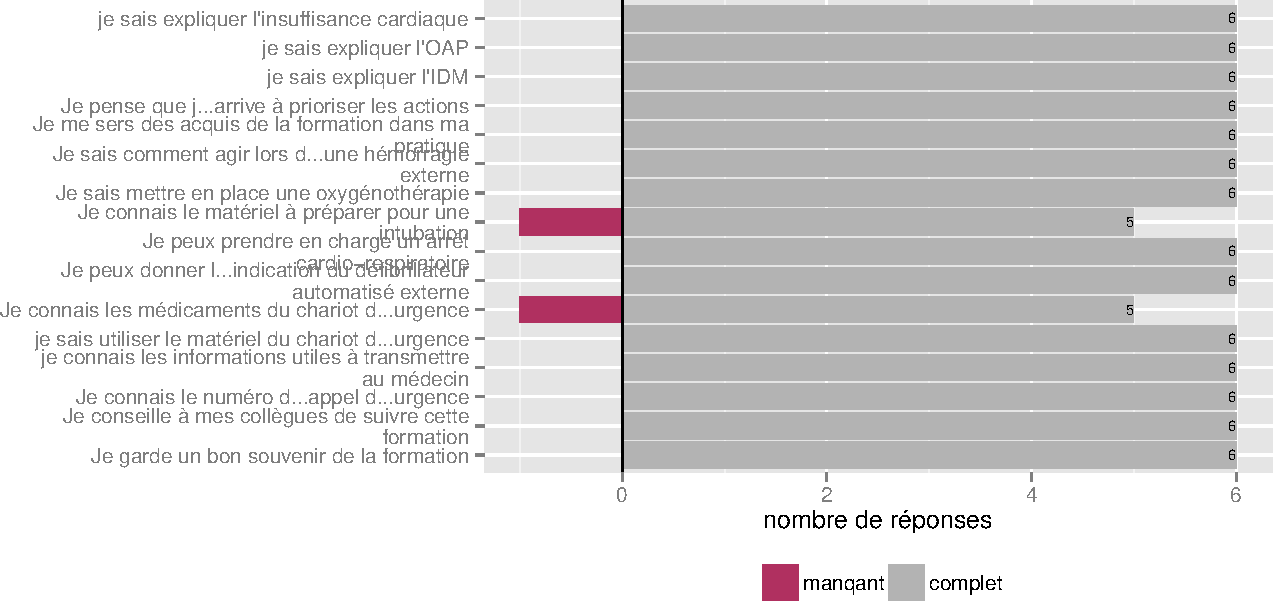
\includegraphics{./questionaire_distance_files/figure-latex/test-1.pdf}
\end{figure}

\begin{Shaded}
\begin{Highlighting}[]
\KeywordTok{likert.heat.plot}\NormalTok{(l, }\DataTypeTok{text.size =} \FloatTok{2.5}\NormalTok{)}
\end{Highlighting}
\end{Shaded}

\begin{figure}[htbp]
\centering
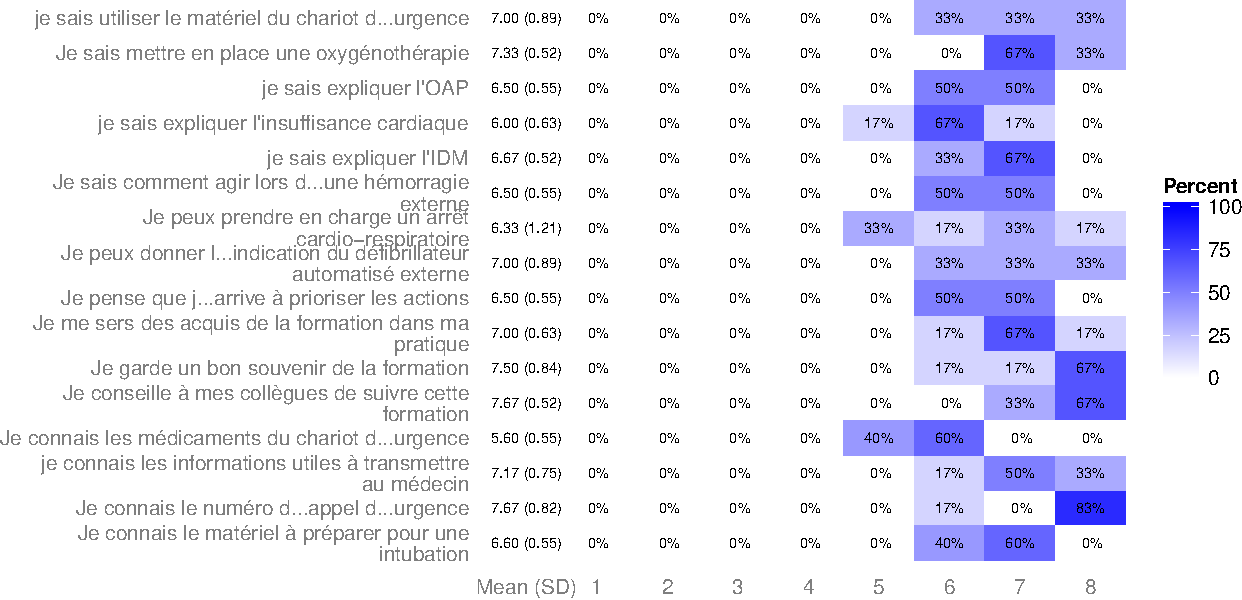
\includegraphics{./questionaire_distance_files/figure-latex/test-2.pdf}
\end{figure}

\begin{Shaded}
\begin{Highlighting}[]
\KeywordTok{likert.density.plot}\NormalTok{(l)}
\end{Highlighting}
\end{Shaded}

\begin{figure}[htbp]
\centering
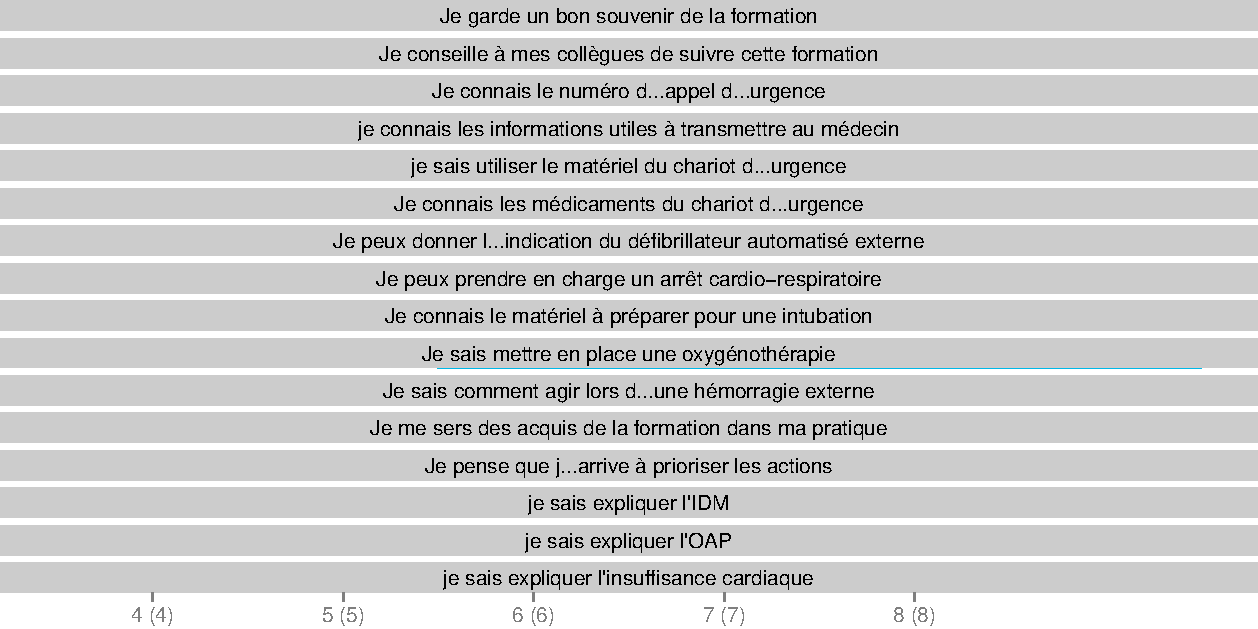
\includegraphics{./questionaire_distance_files/figure-latex/test-3.pdf}
\end{figure}

\begin{Shaded}
\begin{Highlighting}[]
\NormalTok{l =}\StringTok{ }\KeywordTok{likert}\NormalTok{(d, }\DataTypeTok{nlevels =} \DecValTok{8}\NormalTok{)}
\KeywordTok{plot}\NormalTok{(l)}
\end{Highlighting}
\end{Shaded}

\begin{figure}[htbp]
\centering
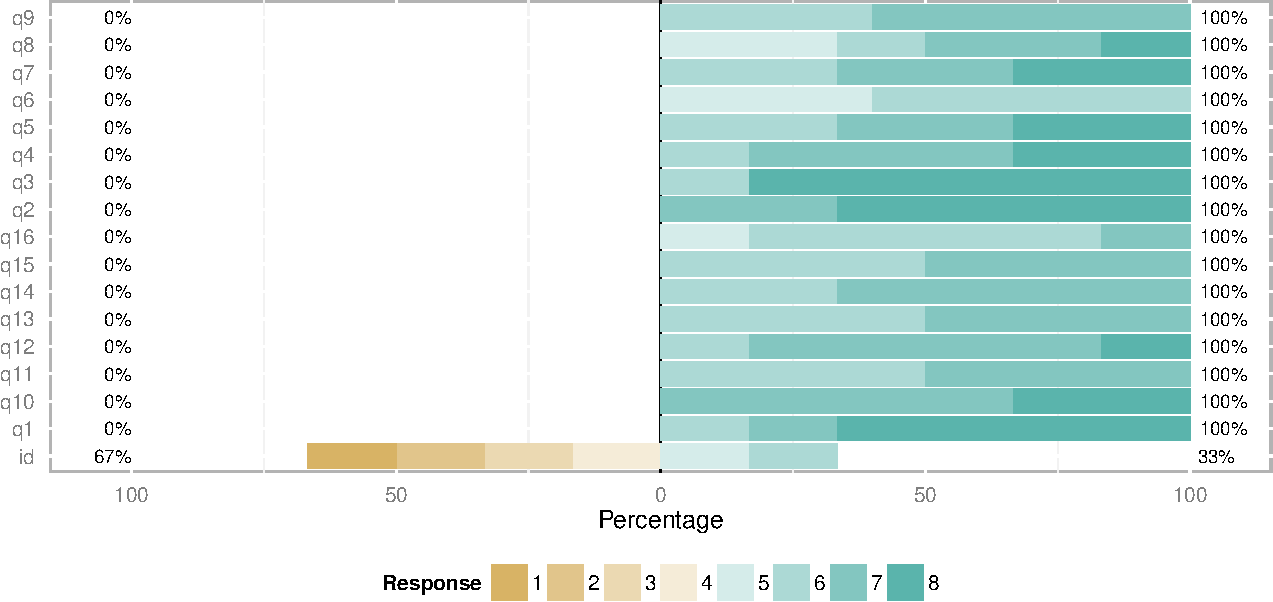
\includegraphics{./questionaire_distance_files/figure-latex/test-4.pdf}
\end{figure}

\subsection{Rotation image}\label{rotation-image}

\paragraph{utilisation de heat plot}\label{utilisation-de-heat-plot}

L'argument \emph{out.extra=`angle=90'} autorise la rotation de l'image.
Fonctionne bien en \textbf{.pdf} mais pas au format word (pas
d'affichage). En mode HTML la rotation ne se fait pas mais l'affichage
reste normal.

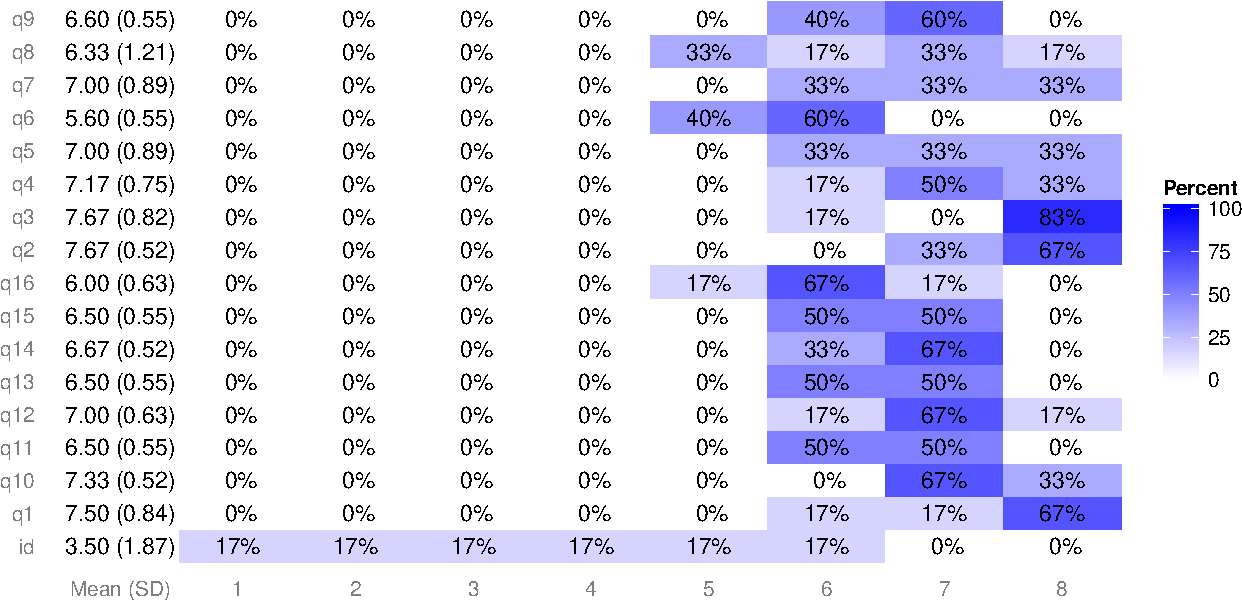
\includegraphics[angle=90]{./questionaire_distance_files/figure-latex/rot-1}

\end{document}
